\chapter{Event reconstruction}\label{chap:Event_reconstruction}
\textit{This chapter describes how the physical objects are reconstructed using the combined information coming from the CMS subdetectors. The electron and photon reconstruction is described in Section \ref{sec:electron_photon}, the muon reconstruction in Section \ref{sec:muon}, the tau reconstruction in Section \ref{sec:taus}, the jet and b-tagged jet reconstruction in Section \ref{sec:Jets} and finally the missing transverse energy reconstruction in Section \ref{sec:MET}.}
\section{Electron and photon reconstruction}\label{sec:electron_photon}
The beginning of reconstruction of electron or photon is to cluster its energy deposition in the ECAL and then to estimate its real energy and position from this information.
In fact that an electrons can radiate bremsstrahlung photons when it traverses the material between the interaction point and the ECAL, that photons can convert into electron pairs when it traverses the material, which in turn can radiate bremsstrahlung photons. The bending of the electron in the CMS magnetic field results in a spread of energy for both electron and photon in the large $\phi$ direction in the ECAL. The energy of electron or photon can be collected by making a cluster of ECAL clusters along a $\phi$ road  which is called a super-cluster (SC).
Finally, the presence a track which match to the SC in ECAL allows one to distinguish a electron from a photon.
\subsection{Clustering}\label{subsec:clustering}

There are two algorithms to cluster the electromagnetic shower in the ECAL. One is Island algorithm which is designed to search for small deposits of energy in individual clusters, for example when making a calorimetric isolation cut, the basic clusters of the Island algorithm are more appropriate objects to work with.
Another is Hybrid algorithm which is designed to reconstruct relatively high energy electrons in the barrel (for electrons with $E_{T}$ > 10 GeV). The details of these two algorithms are described below.

\subsubsection{The Island algorithm}\label{subsubsec:Island}

The island algorithm starts by searching for crystals which have transverse energy above a certain threshold. These crystals are called ``seeds'' and are listed by decreasing energy. The algorithm then loops over seeds and removes those seeds that are adjacent to higher energy ones, after this process only the seeds with local maximum transverse energy remained. Then starting from the most energetic seed, the algorithm collects crystals belonging to a certain cluster (which contains the seed). The sequence is sketched in Figure \ref{fig:Cluster_Island}: starting from the seed position, the algorithm moves in both directions in $\phi$ and collects all crystals until it sees a rise in the energy or a hole (a crystal has very low energy which comparable to a noise). Then it moves one step in $\eta$ and makes another $\phi$ search. The $\eta$-steps are stopped when a rise in energy or a hole is encountered. When one direction in $\eta$ is completed, the algorithm goes back to the seed position and works in the other $\eta$ direction. All the collected crystals are marked as belonging to that one cluster and cannot be used anymore. This procedure guarantees that there is no double counting of crystal energy.

\begin{figure}[h!]
\begin{center}
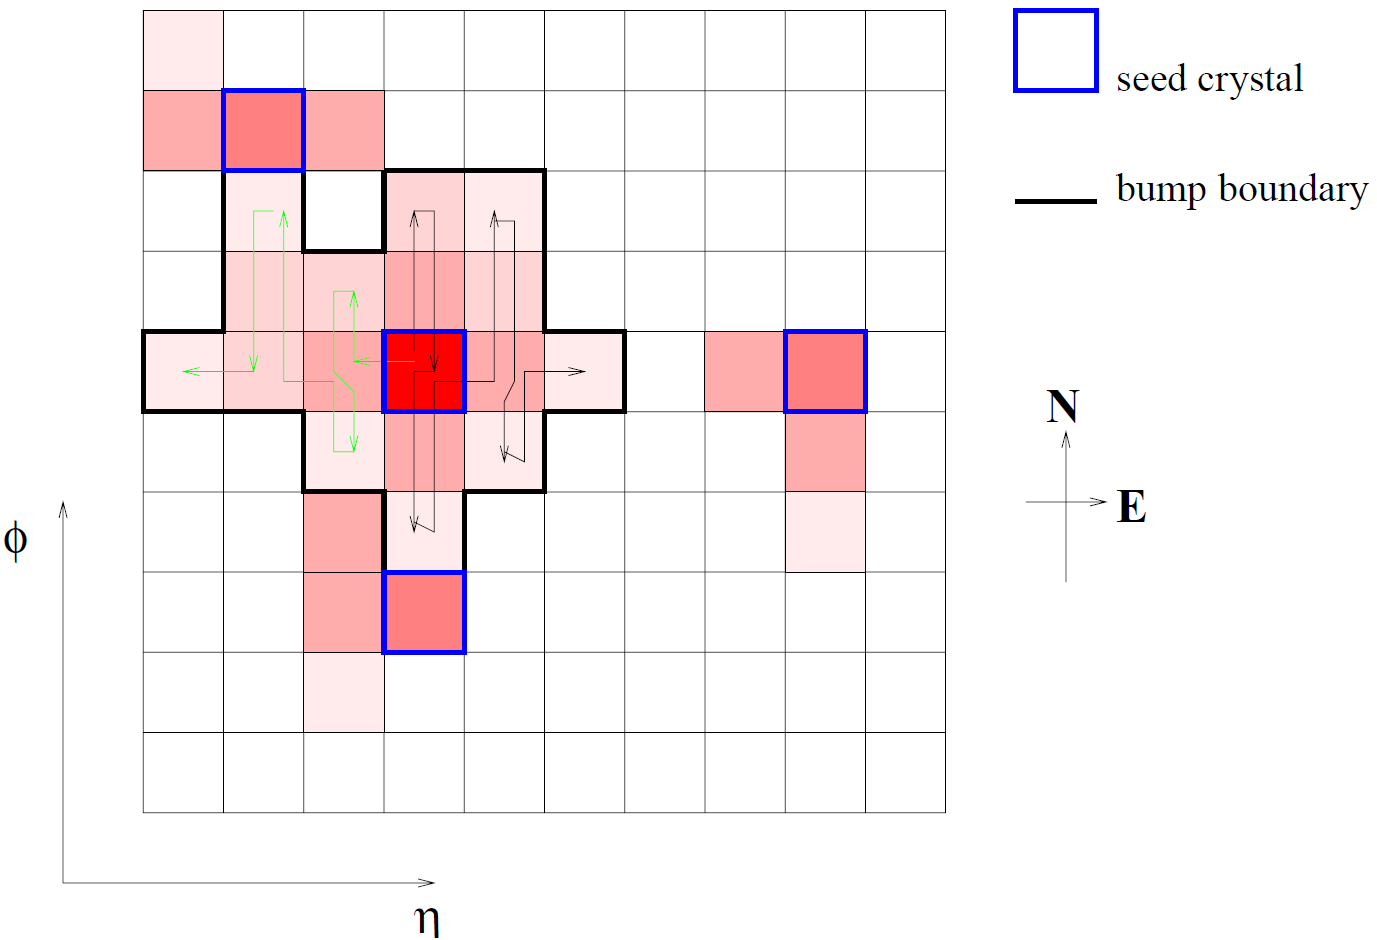
\includegraphics[width=0.9\textwidth]{figures/Reconstruction/Electron_photon/Island.png}
\caption{Illustration of the Island clustering algorithm in the barrel ECAL \cite{CMS-Note-2001-034}.}
\label{fig:Cluster_Island}
\end{center}
\end{figure}

Because much of the endcap is covered by a preshower device with two planes of silicon strip readout. The energy deposited in the preshower detector (which is about 3 $X_{0}$ thick) needs to be added to the crystal clusters. A preshower cluster is constructed in each plane, in front of each crystal cluster. The search area in the preshower is centred on the point determined by extrapolating the crystal cluster position to the preshower plane in the direction of the nominal vertex position.

There are only one parameter for the island algorithm which is the $E_{T}$ threshold of the seed. This value has to be a trade-off between an optimal energy resolution and cutting off noisy hits, low pile up energy as well as keeping the execution time low.

\subsubsection{The Hybrid algorithm}\label{subsec:Hybrid}

In the case of a unconverted photon shower or electrons in test beam conditions, the summed energy from fixed arrays of crystals seems to consistently give better results in terms of energy resolution, than energy sums of crystals collected dynamically according to a cluster finding algorithm. This seems to be because containment variation as a function of impact position is amplified by dynamic cluster finding (e.g. at the shower borders, where energy depositions are
comparable to noise, energy belonging to the shower may be noise-suppressed, or a large noise fluctuation may fake the presence of a secondary seed). The Hybrid algorithm attempts to use the $\eta$-$\phi$ geometry of the barrel crystals to exploit the knowledge of the lateral shower shape in the $\eta$ direction (taking a fixed domino of three or five crystals in $\eta$), while searching dynamically for separated (bremsstrahlung) energy in the $\phi$ direction.

The algorithm starts from a seed crystal (the maximum energy crystal in the region being searched which must also satisfy the condition $E_{T}$> $E_{T}^{hybseed}$), 1$\times$3 crystal dominoes are made, each with their central crystal aligned in $\eta$ with the seed crystal. If the energy of the central crystal of a domino
is greater than $E^{wing}$ then a 1$\times$5 domino is used. This making of dominoes proceeds $N_{step}$ crystals in each $\eta$ direction from the original seed crystal. Dominoes with energy less than $E^{thresh}$ are eliminated. The domino construction step of the algorithm is illustrated in Figure \ref{fig:Cluster_Hybrid}.

\begin{figure}[h!]
\begin{center}
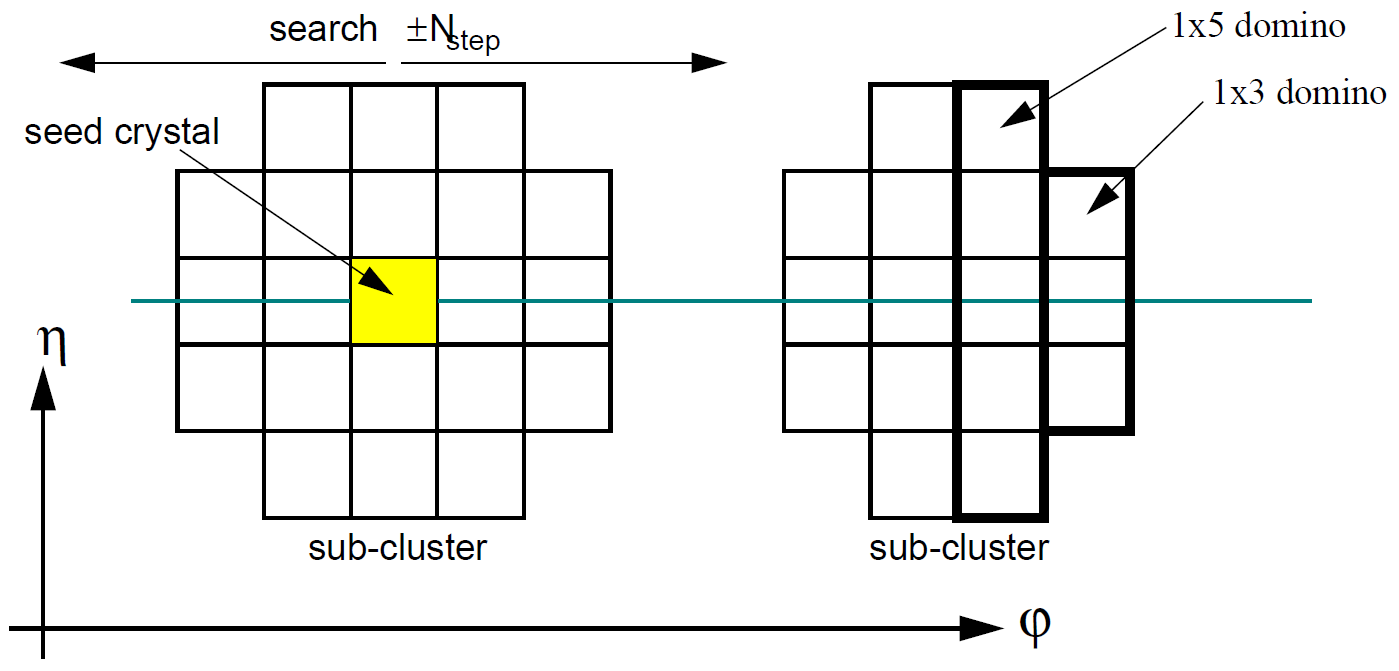
\includegraphics[width=0.9\textwidth]{figures/Reconstruction/Electron_photon/Hybrid.png}
\caption{Domino construction step of Hybrid algorithm \cite{CMS-Note-2001-034}.}
\label{fig:Cluster_Hybrid}
\end{center}
\end{figure}

The dominoes are then clustered in $\phi$. Each distinct cluster of dominoes is required to have a seed domino with energy greater than $E^{seed}$. The default values of the control parameters for Hybird algorithm are shown in Table \ref{tab:Hybrid_parameters}.

\begin{table}[htp]
%\small
\caption{Default values of control parameters for Hybrid algorithm .\label{tab:Hybrid_parameters}}
\begin{center}
  \begin{tabular}{|l|c|c|}
    \hline
    Parameter description                                            & label used in text& default value  \\  \hline\hline
    Minimum $E_{T}$ for Hybrid super-cluster seed crystal            & $E_{T}^{hybseed}$ & 1 GeV \\  \hline
    Number steps (crystals) for search in $\phi$ (in each direction) & $N_{step}$        & 10     \\ \hline
    Threshold for using 1$\times$5 crystals (rather than 1$\times$3) & $E^{wing}$        & 1 GeV  \\ \hline
    Threshold for using domino                                       & $E^{thresh}$      & 0.1 GeV  \\ \hline
    Minimum domino to make a disconnected subcluster                 & $E^{seed}$        & 0.35 GeV \\ \hline
  \end{tabular}
\end{center}
\end{table}





\subsection{Super-cluster (SC)}\label{subsec:super-cluster}

A possible approach to recollecting energy radiated by an electron or photon that falls outside the main shower cluster is to build a cluster of clusters. In much the same way as cluster energy is clustered at the level of calorimeter cells, non-overlapping clusters can in turn be clustered into SC. The procedure is started by searching for the most energetic cluster (seed cluster) and then by recollecting the others based on some geometric criterion, e.g. a fixed search area around the seed cluster. In a purely axial magnetic field the clusters belonging to radiation from a single electron will be nicely aligned in narrow $\eta$ region, but spread in $\phi$. In this case, one can hope that collecting all the clusters in a narrow $\eta$ window, whose size is dictated by the $\eta$ position resolution of the detector, it is possible to recover most of the radiated energy (at least all that is clustered), as illustrated in the Figure \ref{fig:Super-cluster}.

\begin{figure}[h!]
\begin{center}
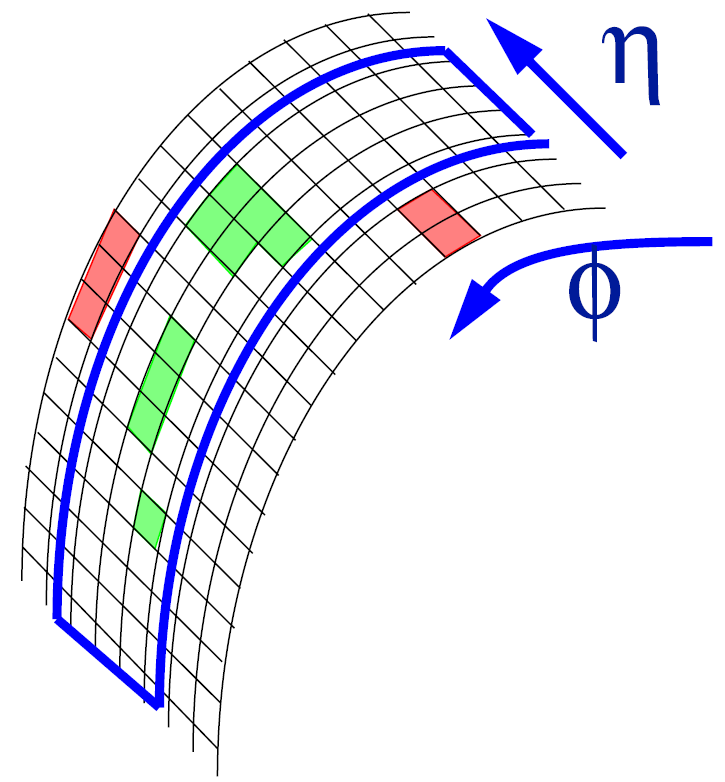
\includegraphics[width=0.5\textwidth]{figures/Reconstruction/Electron_photon/SuperCluster.png}
\caption{Illustration of a super-cluster algorithm collects all clusters which satisfies a given geometric condition (e.g. lying in a certain region around the seed cluster) \cite{CMS-Note-2001-034}.}
\label{fig:Super-cluster}
\end{center}
\end{figure}

%After obtaining ECAL SC, they can be used for driving the finding of pixel seeds for the primary electron tracks.

\subsection{Position measurement}\label{subsec:electron_photon_position}

A simple position measurement of the shower can be obtained by calculating the energy weighted mean position of the crystals in the cluster. However, there are two issues need to be considered in more detail. Firstly, the meaning of \textit{crystal position} needs to be defined. The crystals in the CMS ECAL are quasi-projective, and do not exactly point to the nominal interaction vertex. So the lateral position ($\eta$,$\phi$) of the crystal axis depends on depth as illustrated in Figure \ref{fig:cluster-position}. A depth \textit{tmax} thus needs to be defined and it is also dependent on particle type, e.g. electron showers have a short radiation length comparing with photon showers.

\begin{figure}[h!]
\begin{center}
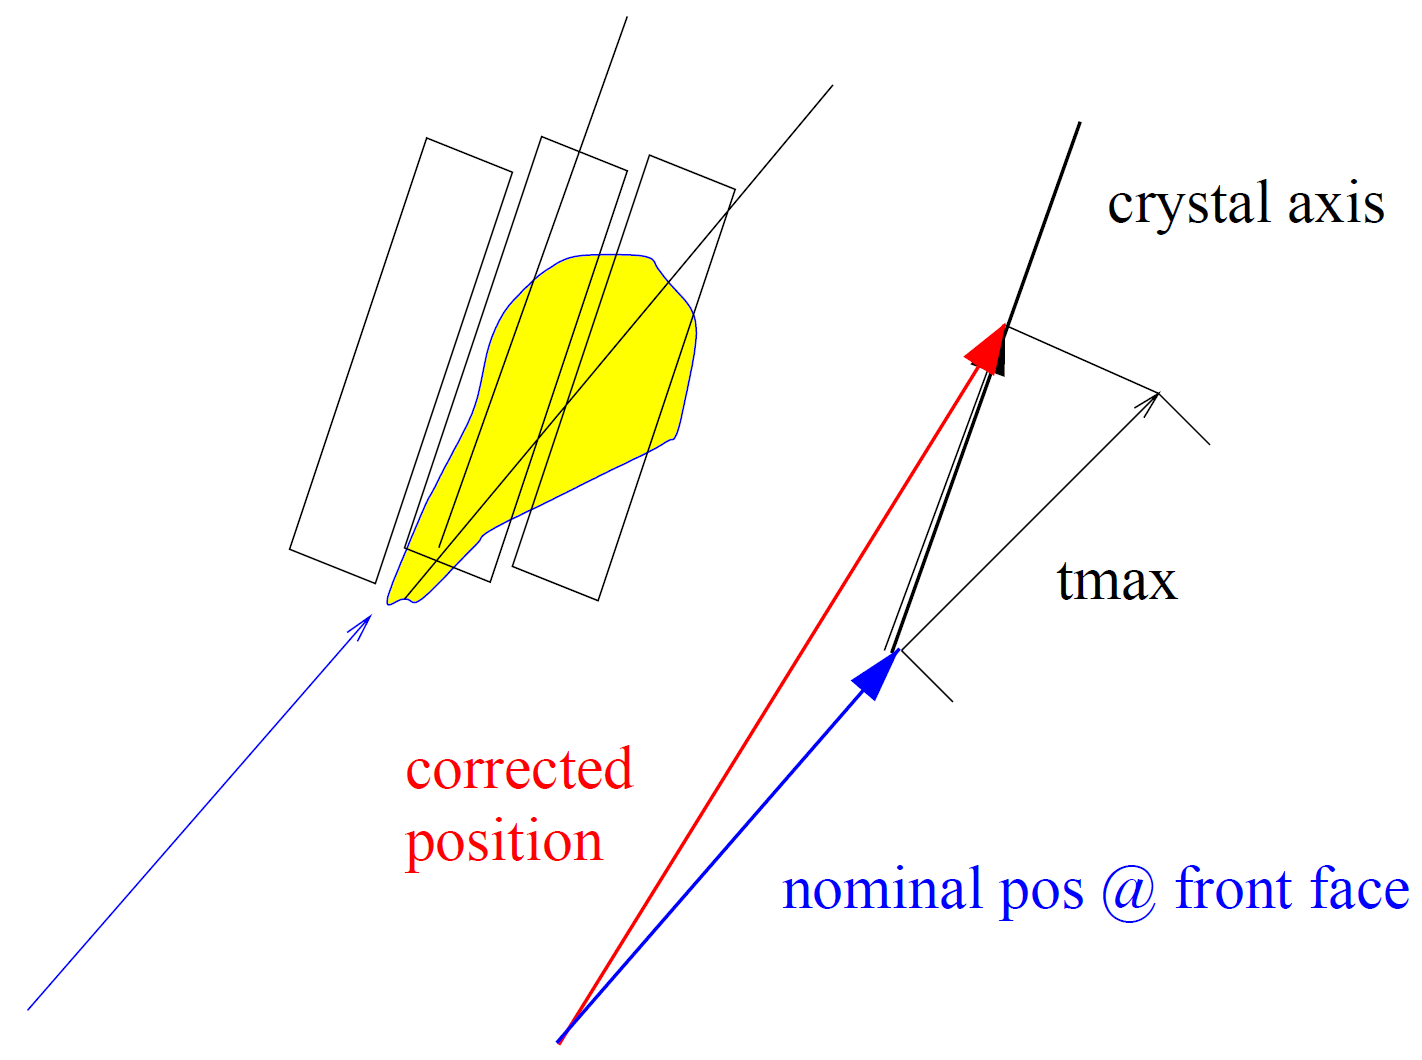
\includegraphics[width=0.5\textwidth]{figures/Reconstruction/Electron_photon/Position.png}
\caption{Illustration of the crystal offpointing \cite{CMS-Note-2001-034}.}
\label{fig:cluster-position}
\end{center}
\end{figure}


The second issue is related to the lateral shower shape. Since the energy density does not fall away linearly with distance from the shower axis, but rather exponentially, a simple energy weighted mean of crystal energies is distorted and the measured position is biased towards the centre of the crystal containing the largest energy deposit. Therefore, a new algorithm is used which delivers almost as good precision by calculating the weighted mean using the logarithm of the crystal energy:

\begin{equation}
x=\frac{\Sigma x_{i}\cdot W_{i}}{\Sigma W_{i}}
\label{eq:logarithm}
\end{equation}

where $x_{i}$ the position of crystal i, and $W_{i}$ is the log weight of the crystal which is the log of the fraction of the cluster energy contained in the crystal, calculated with the formula:

\begin{equation}
W_{i}=W_{0}+ln(\frac{E_{i}}{\Sigma E_{j}})
\label{eq:log_fraction}
\end{equation}

where the weight $W_{i}$ is constrained to be positive otherwise it is set to zero. $W_{0}$ controls the smallest fractional energy that a crystal can have and still contribute to the position measurement. Its default value which is obtained after optimization studies is 4.2, so that crystals in the cluster containing
more than 1.5\% of the cluster energy will contribute to the position measurement.

\subsection{Electron reconstruction}\label{subsec:electron_reco}
In order to reconstruct electron we need to find a track in the tracker which match to the SC and of course this is not required for photon. To search for the track, four steps are involved: the track seed selection, the track building and the track fitting (the last two are usually referred to as ``tracking'') and the track SC matching. They are described below.

\subsubsection{Track seeding}\label{subsec:track_seeding}
Track seeds are the starting point for the track reconstruction which are built from doublets or triplets of hits in the pixel detector. There are two
different approaches for track seeding: the ECAL driven seeding and the tracker driven seeding.

For the ECAL driven seeding, the procedure starts from a SC in ECAL, with at least 4 GeV of transverse energy and a veto of 0.15 on the ratio of hadronic energy to SC energy. Hits in the pixel layers are predicted by propagation of the energy weighted mean position of the SC (see Section \ref{subsec:electron_photon_position}) backward through the magnetic field under both charge hypotheses towards the pixel detector. The reason for this step is that the SC and pixel matching takes advantage of the fact that the energy weighted average impact point of the electron and associated bremsstrahlung photons, as calculated using information from the SC in the ECAL, coincides (assuming a successful collection of photons) with the impact point that would have been measured for a non-radiating electron of the same initial momentum. It is this space-point that the position measurement of the SC attempts to determine. This point can be propagated back through the field to obtain an estimate of the direction of the electron at the vertex, and the hit positions expected in the pixel detector. Since most of the tracker material lies after the pixel detector, most electrons do not radiate significantly before it, and most photon conversions take place after it.

Next a first compatible hit is looked for in the innermost pixel layer within a loose $\Delta\phi$ window and loose $\Delta z$ interval, when a first compatible hit is found a new estimate for the z coordinate of the primary track vertex is calculated combining the found pixel hit and calorimetry information in the \textit{Rz} plane. The predicted trajectory is then propagated to look for a second pixel hit in the next pixel layer(s), within some narrower $\Delta\phi$ and $\Delta z$ windows. If the first two hits are matched with the prediction from the SC, then the seed is selected.

For the tracker driven seeds, they are selected from tracks that were reconstructed with the Kalman filter (KF) algorithm \cite{Hamilton:2016qnl}. This algorithm is not suited for electrons that emit bremsstrahlung photons since the curvature of the track changes in that case. All seeds of KF tracks that match a SC in the ECAL and pass a matching criterion are selected.

The choice of two approaches is analysis dependent, a seeding strategy could be preferred with respect to the other. For example in the search for high mass resonances decaying in dielectron final state (see Chapter \ref{chap:Zprime}), the ECAL driven seeding is required at selection level.


\subsubsection{Tracking}\label{subsec:tracking}

Once the track seed has been obtained, the tracking procedure can take place. The tracking procedure consists of the  ``track building'' which outwards from the seed and the combinatorial track finder method (CTF) \cite{track_jinst} is used (which is an extension of the standard KF method), followed by the ``track fitting'' which uses a Gaussian sum filter (GSF) method \cite{Anuar:2015lxt} in a backward fit. For the track building the CTF method makes use of a specific Bethe-Heitler (BH) \cite{PhysRevA.87.062107} model (modeling the electron energy losses during track building) when collecting matching hits in successive silicon layers, with a tolerance of 1 layer without hits. Since the distribution of the energy loss after the BH model is non-Gaussian, fitting the track with the KF algorithm that uses Gaussian distributions will not give good results. For this reason, the GSF algorithm models the BH energy loss distribution as a sum of six Gaussian distributions with different means, widths and amplitudes. After passing through a layer, six new trajectory components are generated with the weight according to the weight of the initial trajectory multiplied by the weight of the Gaussian component in the BH energy loss distribution estimation. To limit the maximal number of followed trajectories to 12, the ones with low weight are dropped or merged if they are similar. Finally, the track parameters obtained have their uncertainty distributed according to the sum of Gaussian distributions from the trajectory components.

One of the great benefit of the GSF tracks comes from the combined facts that hits are collected efficiently along the full trajectory through the tracker volume, and that meaningful track parameter errors are available at both track ends. Thus, a good estimation of the electron track parameters at ECAL entrance is made available.
Moreover, the fractional amount of momentum carried away by bremsstrahlung photons can be evaluated from the outermost and innermost track parameters. This will be very useful information in distinguishing various electron patterns, to improve electron energy measurements and electron identification.


\subsubsection{Track-supercluster matching}\label{subsec:track_sc_matching}

In order to build GSF electron candidates, a track has to be associated to a SC.

For ECAL driven tracks, the difference between energy weighted position of SC and the position of the track at the SC which is the extrapolated from the innermost track should be smaller than 0.02 in the $\eta$ direction and 0.15 rad in the $\phi$ direction.

For tracker driven tracks a multivariate technique, using a boosted decision tree (BDT), is used which combines track observables and SC observables to get a global identification variable. For a successful matching, the track-SC combination should have a value which higher than a threshold of this variable.

\medskip
A schematic view of the electron reconstruction procedure, considering also multiple bremsstrahlung emissions, is shown in Figure \ref{fig:ele_reco}.
\begin{figure}[!htb]
  \begin{center}
    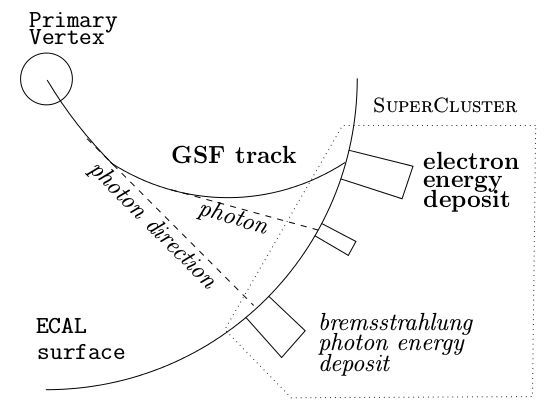
\includegraphics[width=0.5\textwidth]{figures/Reconstruction/Electron_photon/electron_reco_scheme.png}
    \caption{Schematic view of an electron reconstructed in CMS. The track is reconstructed by the GSF algorithm taking into account the trajectory kinks due to energetic bremsstrahlung photon emission. The energy deposits belonging to the emitted photons are collected together to the electron cluster by the clustering algorithm.\label{fig:ele_reco}}
  \end{center}
\end{figure}

\subsection{Photon reconstruction}\label{subsec:photon_reco}
The photon is the simplest electromagnetic object. Any reconstructed SC with $P_{T}>$ 10 GeV is considered as a photon candidate \cite{Soffi2016}. In order to reduce the fake photon from other object like electron, hadron and jet, the most important tool to be used is isolation requirement. Fake photon due to jets can usually be rejected by looking for additional energetic particles in a cone around the reconstructed ECAL cluster. Charged particles like electron, pions and kaons can be detected in the tracker or in the calorimeter. Neutral pions and other particles decaying to photons can be detected in the ECAL. The hadron calorimeter is important for detecting hadrons which do not efficiently reconstructed in the tracker, particularly at high pseudorapidity or particles like neutrons. Therefore, the basic isolation variables considered are based on charged tracks reconstructed in the tracker, electromagnetic energy deposits observed in the ECAL, and hadronic energy deposits
in the HCAL.

Photon candidates which are converted (produce an electron pair) in the material upstream ECAL are tagged using an algorithm which searches for conversion
tracks matching the ECAL SC, as will be described in the following subsection.
\subsubsection{Photon conversion}\label{subsec:photon_conversion}
A large number of photons originating from the primary interaction vertex convert in the tracker material. Identification of converted photons allows a better choice of energy clustering algorithm. The approach to reconstruct conversion track pairs are similar with standard tracks reconstruction as described before. The energy deposits in the ECAL are used as a starting point for inward track seed finding. For each cluster both positive and negative charge hypotheses are tried. The final opposite-charge track pairs are combined together and asked to satisfy the photon conversion topology.

Before finishing this section it is worth mention that at analysis level many other variables (like shower shape, isolation and so on) will be used to distinguish electron and photon from jet efficiently. Several variables are helpful in this task and can be combined in a set of selection criteria used by the CMS analyses.

\section{Muon reconstruction}\label{sec:muon}
The muon reconstruction use the information from muon system and silicon tracker. For the muon which is reconstructed only using muon system information is called ``standalone muon''. The muon which is reconstructed by combining the information coming from the muon system inwards to the inner tracker are referred to as ``global muon candidates''. Finally, muon candidates reconstructed by combining the information coming from the inner tracker outward to the muon station are referred to as ``tracker muon candidates''. The global muon reconstruction is especially efficient for muons leaving hits in several muon stations, the tracker muon reconstruction
is more efficient for low $P_{T}$ muon candidates. The efficiency for reconstructing a muon as global or tracker muon is as high as 99\%.

\subsection{Standalone muon reconstruction}\label{subsec:Standalone_muon}

The standalone muon reconstruction uses only information from the muon detectors (the silicon tracker is not used). Both tracking detectors (DT and CSC) and RPCs (see Section \ref{subsec:CMS_muon}) participate in the reconstruction. Despite the coarser spatial resolution, the RPCs complement the tracking chambers, especially where the geometrical coverage is problematic (mostly in the barrel-endcap overlap region). The reconstruction of muon tracks in the muon system starts from seeds, generated by the DT and the CSC, which are fitted to produce track segments. The state vectors (track position, momentum, and direction) associated with the segments found in the innermost chambers are used to seed the muon trajectories, working from inside to outside using the KF technique. The predicted state vector at the next measurement surface is compared with existing measurements and will be updated accordingly. In case no matching hits are found (e.g. due to detector inefficiencies, geometrical cracks) the search is continued in the next station. The track parameters and the corresponding errors are updated at each step. The procedure is iterated until the outermost measurement surface of the muon system is reached. Then a backward KF is applied, working from outside to inside and the track parameters are defined at the innermost muon station. Finally, the track is extrapolated to the nominal interaction point and a vertex-constrained fit to the track parameters is performed.

\subsection{Global muon reconstruction}\label{subsec:Global_muon}
The reconstruction of global muon consists extending the standalone muon to include hits in the silicon tracker. It starts with extrapolating muon trajectory from the innermost muon station to the outer tracker surface and taking into account the muon energy loss in the material as well as the effect of multiple scattering. Silicon layers compatible with the muon trajectory are then determined and a region of interest (ROI) within them is defined in which the track reconstruction will be performed. The determination of the ROI is based on the standalone muon parameters and their corresponding uncertainties. The a well defined ROI can improve the reconstruction efficiency, reduce fake rate and save CPU reconstruction time.

Inside the ROI, initial candidates for the muon track (regional seeds) are built from pairs of reconstructed hits. Starting from the regional seeds, a track-reconstruction algorithm, based on the KF technique is used to reconstruct tracks from outside to inside. After the tracker track is obtained, it will be asked to match with standalone muon. If there is a suitable match between the tracker track and the standalone muon track, a final fit is performed all over the hits (otherwise no global muon is produced). However it is also possible to combine only a subset of the hits for the final fit. In particular, choosing a subset of the muon hits provides a better momentum resolution for high energy muons, when the measurements in the muon system are frequently contaminated by electromagnetic showers. Finally, the global muon reconstruction ends with the matching of the global muon track and the energy deposits in the calorimeters.

\subsection{Tracker muon reconstruction}\label{subsec:Tracker_muon}
For low $P_{T}$ muons (below 6-7 GeV), large fraction of them does not leave enough hits in the muon detector to be reconstructed as standalone muons. In addition, some muons can escape in the gap between the wheels. Therefore a complementary approach which starts from the tracker tracks to reconstruct muon has been
designed \cite{muon_reco_2} and hence improve the muon reconstruction efficiency. The algorithm starts extrapolating each reconstructed tracker track outward to other subdetectors like ECAL, HCAL and muon system. After collecting the associated signals from each subdetector, the algorithm gives a decision if the tracker track is produced by a muon according to how well the observed signals fit with the hypothesis. By the way, if the extrapolated track matches at least one muon segment in the muon detector, the track is qualified as a ``tracker muon''.

\section{Particle-flow algorithm}\label{sec:PF_algorithm}
Before moving forward to describe remaining objects reconstruction, it is needed to give a brief introduction about the particle-flow (PF) algorithm \cite{PF_1,PF_2} in CMS. This algorithm allows to reconstruct stable particles which are called ``PF particles'' (including electron, photon, muon, charged and neutral hadrons) using the combined information from all subdetectors under the form of calorimeter clusters and tracks (individually denoted as PF elements).

Since a single particle can create multiple PF elements, such as a track and several calorimeter clusters. Therefore, a link algorithm is used to link different PF elements to fully reconstruct a PF particle and limit double counting, via computing the distance between the tracks and the calorimeter clusters to determine whether they correspond to the same physical objects. Finally, the individual PF particles are then combined to form more complex objects such as hadronically decaying taus, jets or transverse missing energy.

\section{Tau reconstruction}\label{sec:taus}
Good tau lepton identification is very important for analyses at the LHC that involve searches for Higgs bosons or evidence of SUSY. While tau leptons have a very short lifetime ($2.9\times 10^{-13}s$) and decay right away when they are produced. Therefore, tau leptons are reconstructed from their visible decay products. In
the case of a leptonic decay (about one third of the cases), the electron or the muon is the only reconstructed particle and the standard tools for electron and muon reconstruction (described in the previous sections) are used. For the remaining two thirds of cases, taus decay hadronically with the production of a jet with very specific features which contain one or three charged hadrons (mostly pions) and several neutral pions which decay into two photons immediately. Moveover, jets coming from tau decays are on average more collimated and isolated than quark and gluon jets. The taus with hadronically decay are reconstructed and identified using the hadrons-plus-strips (HPS) algorithm \cite{tau-lepton,tau_2}. The algorithm is designed to reconstruct individual decay modes of the tau by taking advantage of the excellent performance of the PF algorithm in reconstructing individual charged and neutral particles. The HPS algorithm is performed in two steps:
\begin{enumerate}
\item[1.] $\mathbf{Reconstruction:}$ combining charged and neutral particles reconstructed by the PF algorithm that are compatible with specific tau decays and the four-momentum which is expressed in terms of ($P_{T}$, $\eta$, $\phi$, and mass) of tau candidates is computed.

\item[2.] $\mathbf{Identification:}$ discriminators that separate tau decays from quark and gluon jets, and from electrons and muons, are computed. This provides a reduction of misidentified taus from the jet, electron and muon.
\end{enumerate}

The efficiency in identifying hadronically decaying taus is typically between 45\% and 70\% for misidentification rates of a jet as a tau of the order of 1\%. There are some reasons for the hard reconstruction of tau: in LHC the cross section of QCD process is several order of magnitude larger than tau's and the jet is the most important background. Since at least one neutrino is produced during the tau decay, only a fraction of its total momentum is measured. Although tau has lower reconstruction efficiency compared with electron and muon, it is still very important in some analysis, e.g. in Higgs boson related analysis, because the branch ratio of Higgs decays to tau pair is much larger than Higgs decays to electron or muon pair, it makes tau being the most sensitive lepton in Higgs related analysis.

\section{Jet and bjet reconstruction}\label{sec:Jets}

The jet producing cross section is the largest one at the LHC. A well designed jet reconstruction algorithm is important because jets will not only provide a benchmark for understanding the detector, but will also serve as an important tool in the search for physics beyond the standard model (e.g.~searching Z' in di-jets final state). Jets coming from quarks and gluons are reconstructed by PF objects. There are several jet reconstruction methods and the most commonly used is the anti-k$_T$ algorithm \cite{jet_cds}. In order to cluster PF objects into the jets, this algorithm defines two variables, one is the distance ($d_{ij}$) between the PF object ($i$) and the pseudojets ($j$), another is the distance ($d_{iB}$) between the PF object ($i$) and the beam ($B$):
\begin{equation}
d_{ij}=\textrm{min}(k_{ti}^{-2},k_{tj}^{-2})\frac{\Delta^2_{ij}}{R^2}
\end{equation}
\begin{equation}
d_{iB}=k_{ti}^{-2}
\end{equation}
where $k_{ti}$ and $k_{tj}$ are the transverse momenta of the $i$ and $j$ entities respectively, $\Delta^2_{ij}=(\phi_i-\phi_j)^2+(\eta_i-\eta_j)^2$, and $R$ is the cone size parameter which can be chosen in the range from 0.4-0.7 depending on the analyses choices. If the smallest distance is of  $d_{ij}$-type, the entities $i$ and $j$ are combined into a new single entity, while if it is of $d_{iB}$-type, the $i$ entity is considered as a jet and removed from the list of entities. The procedure continues until the entity list is empty. Unlike other jet clustering algorithms, the anti-k$_T$ algorithm produces jets with a conical shape, clustered around the hardest particles and with boundaries resilient with respect to soft radiation.

The raw jet energies are corrected to ensure a uniform response in $\eta$ and an absolute calibration in $P_{T}$. The target of the calibration is that the reconstructed jet energy matches the energy of the generated jet. The correction to the raw $P_{T}$ of the jet can be decomposed in four multiplicative terms \cite{jet_cds}:
\begin{itemize}
\item[$\bullet$] An offset correction, to remove the energy due to particles not involved in the hard-scattering process (pile-up, detector noise);
\item[$\bullet$] A MC calibration factor, which corrects the reconstructed energy to match the generated MC particle jet energy, based on simulations;
\item[$\bullet$] A residual calibration for the relative energy scale, to correct the energy response as a function of the pseudorapidity;
\item[$\bullet$] A residual calibration for the absolute energy scale, to make the energy response uniform as a function of the transverse momentum.\\
\end{itemize}

The final energy resolution for a jet of 100 GeV of $P_{T}$ is around 10\%.

\subsection{b-jet reconstruction}\label{subsec:b-jet}

All the quarks will generate a jet except the top quark which decays before hadronizing. However, the jets from b quark can be distinguished from other jets coming from gluons, light-flavor quarks (u, d, s) and c quark fragmentation using track, vertex and identified lepton information. There are different algorithms to tag b-jets but only the Combined Secondary Vertex (CSV) algorithm is described here since it is the most commonly used in the CMS analyses. Because b hadrons typically have a lifetime of $c\tau \simeq$ 450 $\mu$m, a powerful handle to discriminate between b jets and other jets is the existence of a secondary vertex. A secondary vertex is defined as a vertex sharing less than 65\% of its tracks with the primary vertex and separated radially from the primary vertex with a significance at least 3$\sigma$. In addition, if the radial distance exceeds 2.5 cm and if the mass is compatible with a $K^0$ or greater than 6.5 GeV, the secondary vertex is rejected. The last condition for secondary vertices is that the flight direction of each candidate is in a cone with $\Delta R=0.5$ around the jet direction.
In case no secondary vertex is found (about 35\% of cases for real b-jets), the CSV algorithm can use so-called ``pseudo-vertices'', from tracks whose impact parameter is more than 2$\sigma$ away. If no pseudo-vertex is found, the CSV algorithm proceeds from simple track variables. The list of variables used by the CSV algorithm to identify b-jets are summarized as follows \cite{b_cds}:
\begin{itemize}
\item[$\bullet$] The presence of a secondary vertex, a pseudo-vertex or none of them;
\item[$\bullet$] The flight distance significance between the primary and the secondary (or pseudo-) vertex in the transverse plane;
\item[$\bullet$] The number of tracks at the secondary or pseudo-vertex;
\item[$\bullet$] The ratio of the energy carried by tracks at the vertex with respect to all tracks in the jet;
\item[$\bullet$] The pseudorapidities of the tracks at the vertex with respect to the jet axis;
\item[$\bullet$] The number of tracks in the jet.
%\item The 2D IP significance of the first track that raises the invariant mass above the c quark mass;
%\item The 3D IP significances for each track in the jet.
\end{itemize}

A likelihood ratio to reject c-jets and to reject light-parton jets are combined to form the final CSV discriminator. The efficiency of the CSV algorithm in data and simulations for the medium working point is close to 70\% with a mistagging rate of about 1.5\%.

\section{MET reconstruction}\label{sec:MET}

Neutrinos and other hypothetical neutral weakly interacting particles cannot be detected by CMS. However, some information about their presence can be obtained from
the detection of a momentum imbalance in the transverse plane to the beam axis. The missing transverse energy is noted $\vec{\cancel{E}}_T$, while its magnitude is referred to as $\cancel{E}_T$. The measurement of $\cancel{E}_T$ is strongly relies on the reconstruction of all other physics objects and is sensitive to a wide range of effects: mismeasurement or misidentification of physics objects, detector noise or malfunctions, pileup interactions and so on.

There are several types of $\vec{\cancel{E}}_T$ in CMS and the most widely used is the particle-flow (PF) $\vec{\cancel{E}}_T$, which is the negative vectorial sum over the transverse momenta of all PF particles. A bias in the $\cancel{E}_T$ measurement can be caused by several reasons, such as the non-linearity of the response of the calorimeter for hadronic particles, or the minimum energy thresholds in the calorimeters. In addition, another bias comes from the pile-up interactions and it can be corrected by subtracting the $\vec{\cancel{E}}_T$ by a certain fraction ($f(\vec{v})$) of $\vec{v}$ which is the vectorial $P_{T}$ sum of charged particles associated to each pile-up vertex:
\begin{equation}
\vec{\cancel{E}}_T^{corr} = \vec{\cancel{E}}_T - \sum_{PU} f(\vec{v}) \vec{v}
\end{equation}
Finally, an asymmetry in the $\phi$ variable is observed in data and simulated events, and is found to be related to the number of reconstructed vertices $N_{vtx}$. The $\vec{\cancel{E}}_T$ projection in the $x$- and $y$-directions are independently corrected by some functions of $N_{vtx}$.\\

As mentioned before, the $\vec{\cancel{E}}_T$ measurement \cite{met_cds} strongly relies on the reconstruction of all other physics objects, and is sensitive to a wide range of effects. Artificially large $\cancel{E}_T$ can be measured because of spurious detector signals. Sources of fake $\cancel{E}_T$ include:
\begin{itemize}
\item[$\bullet$] Dead cells in the ECAL;
\item[$\bullet$] Beam-halo particles;
\item[$\bullet$] Particles striking sensors in the ECAL barrel detector;
\item[$\bullet$] Noise from HCAL hybrid photodiode;
\item[$\bullet$] Direct particle interactions with light guides and photomultipliers tubes in the forward calorimeter;
\item[$\bullet$] High-amplitude anomalous pulses in the ECAL endcaps;
\item[$\bullet$] A misfire of the HCAL laser calibration system;
\item[$\bullet$] A defective track reconstruction, from coherent noise in the silicon strip tracker.
\end{itemize}
Dedicated algorithms are used to identify and remove these events with fake $\cancel{E}_T$.

\section{Summary}

This chapter describes how the objects used for analyses are reconstructed in CMS.
The electron and photon reconstruction has been described in details in Section \ref{sec:electron_photon}, while the muon, tau, jet and missing transverse energy reconstructions are described in Sections \ref{sec:muon}-\ref{sec:MET}.
